\chapter{Fundamentals}

\section{Differential Privacy}

Differential Privacy ist ein Verfahren, dass die Privatheit bei interaktiven Anfragen auf Datenbanken schützen kann. Es wurde in \cite{dwork:2006} formalisiert, nachdem gezeigt wurde, dass Anforderungen an Privatheit aus \cite{dalenius:1977} in der Praxis nicht umsetzbar sind. In \cite{dalenius:1977} war die Philosophie, dass ein Angreifer nichts lernen soll, was er nicht auch ohne Zugriff auf die Datenbank hätte lernen können. \textcite{dwork:2006} zeigt, dass diese Definition aufgrund von Hilfsinformationen, die der Angreifer besitzen kann nicht umsetzbar ist. Stattdessen verfolgt \textcite{dwork:2006} mit der Differential Privacy einen Ansatz, bei dem nicht direkt das Wissen des Angreifers einbezogen wird, sondern ob der Angreifer bei einer bestimmten Anfrage mehr über ein Individuum lernen kann, wenn es in der zugrundeliegenden Datenbank ist.

Formal vergleicht Differential Privacy die Wahrscheinlichkeit ein ähnliches Anfrageergebnis zu erhalten, wenn ein Individuum in einer Datenbank ist oder nicht. Je weniger diese Wahrscheinlichkeiten auseinander liegen, desto weniger kann ein Angreifer durch die Präsenz des Individuums in der Datenbank lernen und desto höher ist die Privacy. Die Definition aus \cite{dwork:2006} ist folgende:

\begin{definition}
	\emph{\textbf{$\epsilon$-Differential Privacy}} A \textit{randomized mechanism} $\mathcal{M}: \mathcal{D} \rightarrow \mathcal{R}$ with domain $\mathcal{D}$ and range $\mathcal{R}$ satisfies $\epsilon$-differential privacy if for any two adjacent inputs $d$, $d' \in \mathcal{D}$ and for any subset of outputs $S \subseteq \mathcal{R}$ it holds that $$\Pr[\mathcal{M}(d) \in S] \leq e^{\epsilon} \Pr[\mathcal{M}(d') \in S]$$
\end{definition}

Hervorzuheben ist hierbei noch, dass die Definition keine Anforderungen an die Datenbanken $d, d'$ macht, außer, dass sie benachbart sind, sich also nur in einem Eintrag unterscheiden.

Eine leicht abgeschwächte Version der Definition fügt einen Parameter $\delta$ hinzu, der die Wahrscheinlichkeit repräsentiert, dass die Privatheitsgarantien nicht eingehalten werden. Er sollte demenstprechend sehr klein gewählt werden.\cite{dwork:2014} 

\begin{definition}
	\emph{\textbf{$(\epsilon, \delta)$-Differential Privacy}} A \textit{randomized mechanism} $\mathcal{M}: \mathcal{D} \rightarrow \mathcal{R}$ with domain $\mathcal{D}$ and range $\mathcal{R}$ satisfies $(\epsilon, \delta)$-differential privacy if for any two adjacent inputs $d$, $d' \in \mathcal{D}$ and for any subset of outputs $S \subseteq \mathcal{R}$ it holds that $$\Pr[\mathcal{M}(d) \in S] \leq e^{\epsilon} \Pr[\mathcal{M}(d') \in S] + \delta$$
\end{definition}

Um die Definitionen zu erfüllen wird auf ein Anfrageergebnis von $\mathcal{M}$ Rauschen hinzugefügt. Die Varianz der Verteilung, aus der das Rauschen gezogen wird hängt von der Sensitivität einer Anfrage ab. Sie beschreibt die größtmögliche Veränderung für eine Anfrage, die durch das Hinzufügen oder das Löschen eines Eintrags auftreten kann.\cite{dwork:2006}

\begin{definition}
	\emph{\textbf{L1-Sensitivity}} For $\mathcal{M}: \mathcal{D} \rightarrow \mathcal{R}^{d}$, the L1-Sensitivity of $\mathcal{M}$ is 
	$$
	\Delta \mathcal{M} = \max_{d_1, d_2}{||\mathcal{M}(d_1) - \mathcal{M}(d_2)||}_1
	$$
	for all adjacent datasets $d_1$, $d_2$
\end{definition}

Das Rauschen wird je nach Anwendungsfall aus verschiedenen Verteilungen gezogen. Beispielsweise gibt es den Laplace- oder den Gauss'schen Mechanismus, um numerische Anfragen, beispielsweise Durchschnitt einer Datenbank, privat zu machen. Für Anfragen, die ein Ergebnis aus einer festgelegten Menge liefern sollen, gibt es den Exponentiellen Mechanismus. Dieser bewertet die potenziellen Ergebnisse anhand einer Bewertungsfunktion.\cite{mcsherry:2007}

Bei den Mechanismen ist variiert die Definition der Sensitivität leicht, beispielsweise nutzt der Gauss'sche Mechanismus die $\ell_2$-Norm anstatt der $\ell_1$-Norm, die Intuition, dass es um die maximale Abweichung im Anfrageergebnis durch ein Individuum geht, bleibt jedoch immer erhalten. Darüber hinaus erfüllt der Laplace Mechanismus $\epsilon$-Differential Privacy, der Gauss'sche Mechanismus jedoch nur $(\epsilon, \delta)$-Differential Privacy.\cite[p.261ff]{dwork:2014}

Mit den bisher erwähnten Methoden kann die Privatheit einzelner Anfragen gewährleistet werden. Wenn die gleichen Anfragen aber zum Beispiel mehrfach gestellt werden muss auch das Niveau der Privatheit abnehmen, da der Durchschnitt der einzelnen Anfragen irgendwann gegen den echten Wert konvergiert.\cite[p.42]{dwork:2014} Ein großer Vorteil von Differential Privacy ist, dass sich diese Verringerung der Privatheit abschätzen lässt. Dafür gibt es einige Kompositionstheoreme:

% Kompositionstheoreme einfügen
\begin{itemize}
	\item Group Privacy
	\item Sequential Composition
	\item Parallel Composition
	\item Complex Composition Theorem(?)
	\item Strong Composition Theorem(?)\cite{dwork:2010}
\end{itemize}

Darüber hinaus können Ergebnisse, die durch einen Mechanismus erhalten wurden der Differential Privacy erfüllt, weiterverarbeitet werden, ohne dass die Privatheit weiter kompromittiert wird (\textit{post-processing}).\cite{dwork:2014}

\subsection{Differential Privacy in Machine Learning}
Es gibt verschiedene Punkte, an denen Differential Privacy im Machine Learning ansetzen kann um die Privatheit zu gewährleisten. Jeder Punkt hat verschiedene Vor- und Nachteile, die ich im Folgenden umreiße. Eine Übersicht dazu ist in \autoref{fig:design_principles_dpml} zu sehen.

\begin{figure}[tb]
	\centering
	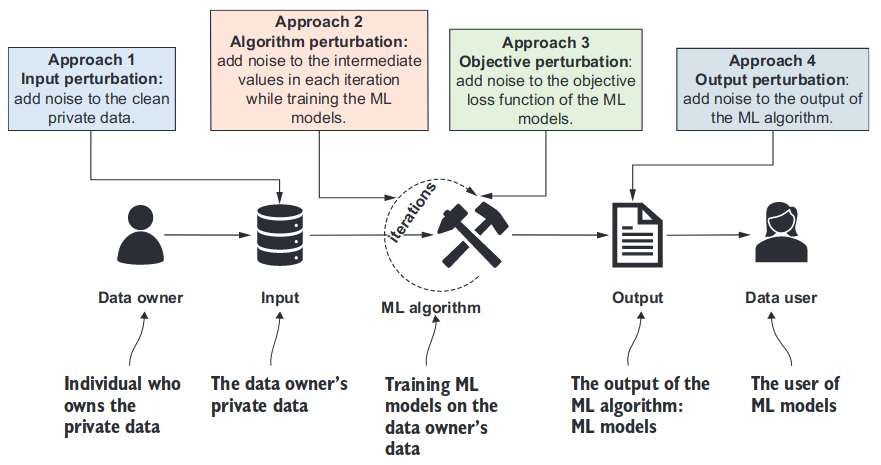
\includegraphics[width=0.7\textwidth]{Bilder/design_principles_dpml.png}
	\caption{Design principles of differentially private ML from \textcite{chang:2023}}
	\label{fig:design_principles_dpml}
\end{figure}

Bei der \textit{Input Pertubation} wird den Trainingsdaten Rauschen hinzugefügt, bevor das Modell mit ihnen trainiert wird. Dieser Ansatz ist ohne weitere Änderungen am Trainingsalgorithmus oder am Modell anwendbar, da der Trainingsalgorithmus dann Daten verarbeitet, die bereits differential private sind und es damit einem \textit{post-processing} entspricht. Das Modell kann danach also problemlos weiterverwendet werden. Ein großer Nachteil ist aber, dass die Anfragen auf den Trainingsdaten im Allgemeinen eine hohe Sensitivität haben und daher viel Rauschen hinzugefügt werden muss.

Die \textit{Algorithm Pertubation} ist das am weitesten verbreitete Verfahren und liegt großen Bibliotheken wie Opacus\cite{yousefpour:2021} und TensorFlow Privacy\cite{tfprivacy} zugrunde. Es kann für iterative Optimierungsverfahren wie Gradient Descent oder die Power Iteration Methode bei einer Principal Component Analysis (PCA) genutzt werden. 

Bei der Anwendung dieses Verfahrens im Gradient Descent wird Differential Privacy auf die Updates der Gradienten angewendet, das heißt diese werden für gewöhnlich auf eine bestimmte Vektornorm gestutzt und dann wird basierend darauf Rauschen addiert. In der Regel muss hierbei deutlich weniger Rauschen hinzugefügt werden, als bei der \textit{Input Pertubation}.\cite{chang:2023} Der \textit{Privacy Loss}, der durch einen Trainingsdurchlauf anfällt, kann mithilfe von Kompositionstheoremen bestimmt werden. Für die Abschätzung wurde das \textit{Strong Composition Theorem}\cite{dwork:2010} genutzt, allerdings konnten \textcite{abadi:2016} mit dem \textit{Moments Accountant} eine deutlich genauere Abschätzung für das Training von Neuronalen Netzen liefern. So können Neuronale Netze mit dem Verfahren bereits mit kleinen Privacy Budgets trainiert werden. Das trainierte Modell kann ebenfalls veröffentlicht werden, da dessen Gewichte die Anforderungen der Differential Privacy erfüllen.

\textit{Objective Pertubation} verändert die Zielfunktion des Trainings. Statt auf die Daten wird während des Trainings Rauschen auf diese Funktion gelegt.

Bei der \textit{Output Pertubation} wird ein nicht-privates Modell trainiert und nur die Ausgabe des Modells verrauscht. Dieses Verfahren hat den großen Nachteil, dass es nicht anwendbar ist, wenn das Modell veröffentlicht werden soll.

\subsection{Individualized Differential Privacy}



\section{Federated Learning}

Federated Learning (FL) ist ein Optimierungsverfahren, bei dem einzelne Clients gemeinsam ein Modell trainieren, ohne dabei ihre eigenen Trainingsdaten mit anderen zu teilen. Dabei initialisiert ein Server ein Modell und seine Parameter. Danach wählt er eine Menge an Clients aus, mit denen in dieser Runde das Modell trainiert werden soll und schickt das Modell an diese. Die Clients optimieren das Modell auf ihren eigenen Daten und schicken das Update an den Server zurück. Dieser aggregiert alle Updates und aktualisiert damit sein Modell. Das ganze Verfahren wird über mehrere Runden wiederholt. 

Die lokale Optimierung und die Aggregation der Updates kann je nach Algorithmus variieren. FedAvg lässt die Clients mehrere Epochen auf ihren eigenen Daten trainieren und gewichtet die Updates bei der Aggregation nach der Menge der Daten, die die einzelnen Clients haben. FedSGD ist ein spezialfall von FedAvg, bei dem die Clients nur für einen Schritt trainieren und das Update dann zurückschicken \parencite{mcmahan:2016}.

\begin{itemize}
	\item cross-device vs cross-silo vs fully distributed
	\item availability of clients (Vorraussetzungen, wie Batterie, Netz, ...)
	\item Non-IID Data
	\begin{itemize}
		\item within a client: can be mitigated by shuffling the datapoints (p.18)
		\item among clients: feature distribution skew, label distribution skew
	\end{itemize}
\end{itemize}

Das verteilte Training kann vor allem zwei Probleme mit sich bringen. Zunächst kann der Overhead für die Kommunikation sehr groß werden, gerade wenn über viele Runden hinweg trainiert wird. Zum anderen kann nicht angenommen werden, dass die Daten über die Clients hinweg IID sind, was die Konvergenz der Algorithmen beeinträchtigen kann. \textcite{karimireddy:2020} versuchen diesem Problem zu begegnen, indem sie in ihrem Algorithmus die generelle Richtung, in die die Clients optimieren, an die Clients schicken und diese sie in ihre Updates einfließen lassen.

\subsection{Data heterogeneity}

\subsection{Privacy model in Federated Learning}
local vs global (trusted server), record vs user level
